\section{Hyperparameter mit Bayesian Search}

%___________________________________________________________________
\begin{frame}{Bayesian Search Erklärt}
\begin{itemize}
    \item Bayesian Search ist eine intelligente Methode zur Optimierung von Hyperparametern.
    \item Ziel: Maximierung der Validierungsgenauigkeit $f(\text{Parameter}) \rightarrow \text{Validation Accuracy}$.
    \item Idee:
        \begin{itemize}
            \item Es wird ein Modell erstellt, das die unbekannte Zielfunktion $f$ abschätzt.
            \item Nach jeder Evaluierung wird dieses Modell mit den neuen Ergebnissen aktualisiert.
            \item Eine \textit{Acquisition Function} wählt die nächsten Parameterwerte aus – als Kompromiss zwischen \textbf{Exploration} (neue Bereiche testen) und \textbf{Exploitation} (bestehende gute Bereiche verfeinern).
        \end{itemize}
    \item Vorteil: Findet gute Parameter mit deutlich weniger Versuchen als Random oder Grid Search.
\end{itemize}
\end{frame}

%___________________________________________________________________
\begin{frame}{Animation zu Bayesian Search}
\centering
\animategraphics[loop, autoplay, controls, width=\imagewidth, height=\imageheight, keepaspectratio]{0.5}{videos/frame_}{000}{006}
\imagesource{\cite{bayes_gif}}
\end{frame}

%___________________________________________________________________
\begin{frame}{Anwendung auf unser Modell}
\begin{columns}[T,onlytextwidth]
    \begin{column}{0.52\textwidth}
        \begin{itemize}
            \item Anstatt zufällig Parameterkombinationen zu testen (Random Search) oder alle möglichen Kombinationen (Grid Search), wurde \textbf{Bayesian Search} verwendet.
            \item Das Modell der Funktion $\text{Validation Accuracy} = f(\text{Hyperparameter})$ wird kontinuierlich angepasst.
            \item Neue Vorschläge für Hyperparameter werden auf Basis bisheriger Ergebnisse erzeugt.
        \end{itemize}
    \end{column}
    \begin{column}{0.45\textwidth}
        \begin{figure}
            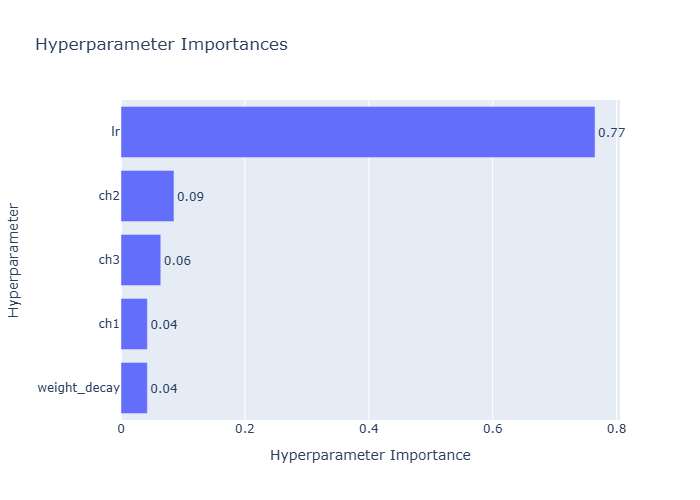
\includegraphics[width=\linewidth, height=\imageheight, keepaspectratio]{param_importances.png}
            \caption{Relative Wichtigkeit der Hyperparameter}
        \end{figure}
    \end{column}
\end{columns}
\end{frame}

%___________________________________________________________________
\begin{frame}{Bayesian Search Ergebnisse}
\begin{figure}
    \centering
    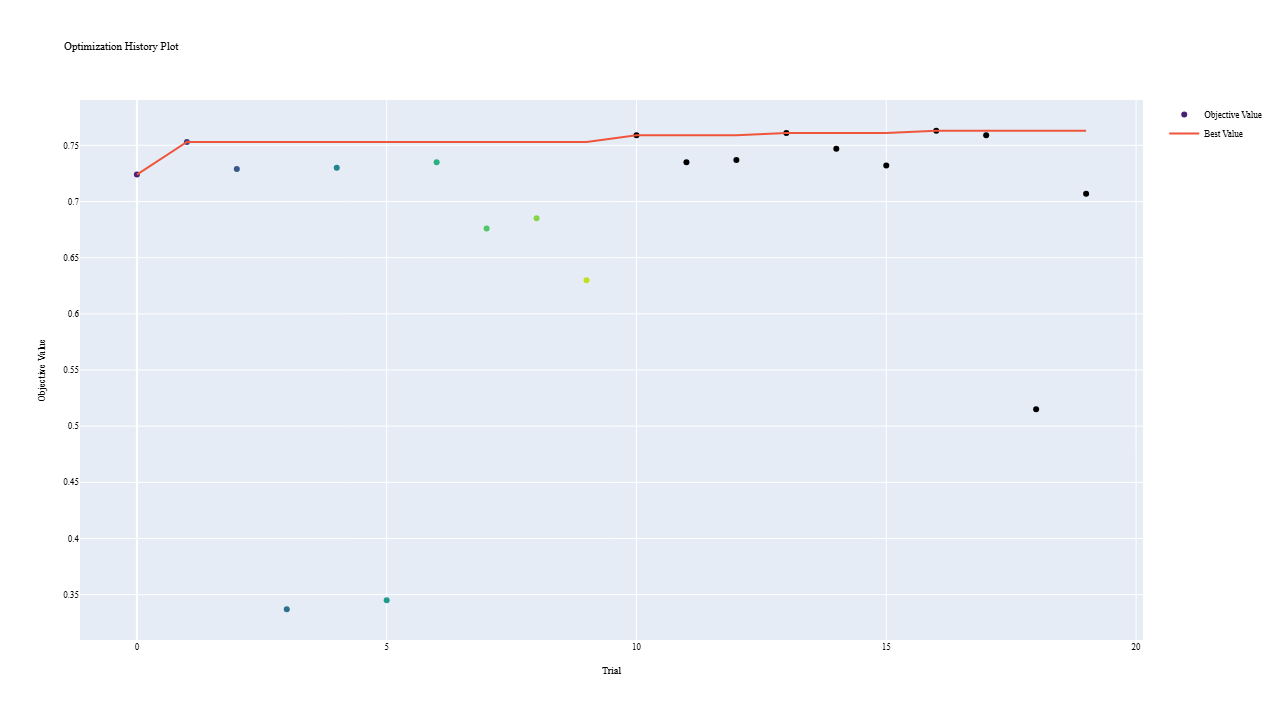
\includegraphics[width=\imagewidth, height=\imageheight, keepaspectratio]{optimization_history.png}
    \caption{Verlauf der Validierungsgenauigkeit über die Trials (je höher, desto besser).}

\end{figure}
\end{frame}
